\documentclass[12pt,phd,times]{pkmthesis}

\usepackage{amsmath,epsfig,graphicx,setspace,url,float}
\usepackage{pstricks,colortab,pifont}
\usepackage{lscape,multicol,multirow,longtable,subfigure}
\usepackage{cite, bm}   
\usepackage{geometry}
\usepackage{array}
\usepackage{algorithm}
\usepackage{multirow}
\usepackage{tabularx}
\usepackage{graphicx} 
\usepackage{subcaption}
\usepackage{booktabs}% Due to this hyberref will not work for references (PKM on 07/07/08)
\usepackage{tikz}
\usetikzlibrary{shapes.geometric, arrows, positioning, fit, backgrounds, decorations.pathreplacing}
\usepackage{cite}
\usepackage[english]{babel}
\usepackage[font=small,labelfont=bf]{caption}              % Added on 26/08/08
%\usepackage{slashbox} 
\usepackage{csquotes}  
\usepackage{threeparttable}
%\usepackage{adjustbox}                    % Added on 24/10/08 (Senthil)
\setlength{\textfloatsep}{1cm}              % Spacing b/w  float and text (PKM 01/11/08)
%..........................................................................................................................................
\normalem                                   % Added on 01/07/08 to avoid underline in the references
\setlength{\abovecaptionskip}{8pt}          % Added on 08/07/08
\setlength{\belowcaptionskip}{8pt}          % Added on 08/07/08
%..........................................................................................................................................
\usepackage{hyperref}
\usepackage{extra_functions}
%\input{pagesetup_pkm_twoside.tex}           % Modified on 06/07/08, 10/07/08, 15/07/08
%\input{pagesetup_pkm_singleside.tex}       % For Single Sided Document 
\input{pagesetup_pkm_middleside.tex}       % Middle alignment 
\raggedbottom                               % o6/08/08  (Remove Unnecessary space b/w paragraphs)
%******************************************************************************************************************************************

\begin {document}
\setcounter{page}{1} \pagenumbering{roman}  % 03/07/08
\onehalfspacing                              % or use \baselineskip 12pt (12, 18 and 24)
%*************************************************** FRONT PAGES**********************************************
%\thispagestyle{empty}
%\pdfbookmark{Title}{Title}
%\begin{center}
\fontsize{15.8pt}{19pt}\selectfont
{\textbf{Next-Day Stock Status Prediction in Fresh Retail \\}}
\vspace*{0.13in}
\emph{\large{A report submitted in fulfillment for the award of the degree of}} \\
\emph{\large{Bachelors of Technology \\}}
\large{in \\}
\large{Information Technology\\}
\large{Bachelors of Technology Project \\}
\large{\textbf{Final Evaluation Report}}

\large{By}\\
 \large{\textbf{Anurag Thakur}} \\ \large{2023IMG-008} \\ \vspace{0.15cm}
 \large{\textbf{Samyak Choudhary}} \\ \large{2023IMG-044} \\ \vspace{0.15cm}
 \large{\textbf{Vibhor Kumar}} \\ \large{2023IMG-054} \\ \vspace{0.25cm}
\large{Under the Supervision of} \\
 \large{\textbf{Dr. Sunil Kumar}} \\
\large{Department of Information Technology}
\end{center}
\begin{figure}[!h]
\centerline{\includegraphics*[width = 3cm]{FrontPages/ABV_IIITM_logo.eps}}
%\centerline{
\epsfig{figure=FrontPages/thapar_logo.eps, []}}
%\centerline{\epsfig{figure=FrontPages/iitg.eps,scale=0.6}}
\end{figure}
\centerline {\large{ABV-INDIAN INSTITUTE OF INFORMATION TECHNOLOGY }}
\centerline{\large{AND MANAGEMENT GWALIOR}} \vspace*{0.05in}
\centerline{\large{GWALIOR, INDIA}} \vspace*{0.05in}
%\centerline{\large{DECEMBER, 2022.}}

%\thispagestyle{empty}
%\clearpage

\thispagestyle{empty}
\pdfbookmark{Title}{Title}
\begin{center}
\fontsize{15.8pt}{19pt}\selectfont
{\textbf{Next-Day Stock Status Prediction in Fresh Retail \\}}
\vspace*{0.13in}
\emph{\large{A report submitted in fulfillment for the award of the degree of}} \\
\emph{\large{Bachelors of Technology \\}}
\large{in \\}
\large{Information Technology\\}
\large{Bachelors of Technology Project \\}
\large{\textbf{Final Evaluation Report}}

\large{By}\\
 \large{\textbf{Anurag Thakur}} \\ \large{2023IMG-008} \\ \vspace{0.15cm}
 \large{\textbf{Samyak Choudhary}} \\ \large{2023IMG-044} \\ \vspace{0.15cm}
 \large{\textbf{Vibhor Kumar}} \\ \large{2023IMG-054} \\ \vspace{0.25cm}
\large{Under the Supervision of} \\
 \large{\textbf{Dr. Sunil Kumar}} \\
\large{Department of Information Technology}
\end{center}
\begin{figure}[!h]
\centerline{\includegraphics*[width = 3cm]{FrontPages/ABV_IIITM_logo.eps}}
%\centerline{
\epsfig{figure=FrontPages/thapar_logo.eps, []}}
%\centerline{\epsfig{figure=FrontPages/iitg.eps,scale=0.6}}
\end{figure}
\centerline {\large{ABV-INDIAN INSTITUTE OF INFORMATION TECHNOLOGY }}
\centerline{\large{AND MANAGEMENT GWALIOR}} \vspace*{0.05in}
\centerline{\large{GWALIOR, INDIA}} \vspace*{0.05in}
%\centerline{\large{DECEMBER, 2022.}}

\thispagestyle{empty}

\clearpage
\thispagestyle{empty}
\pdfbookmark{Dedication}{Dedication}
%\include{FrontPages/Dedication}
\newpage
\thispagestyle{empty}
\clearpage
\thispagestyle{empty}
\pdfbookmark{Certificate}{Certificate}

\begin{center}
{\Large \bf DECLARATION}
\end{center}
\vspace{0.5cm}
\noindent We hereby certify that the work, which is being presented in the report, entitled \textbf{Next-Day Stock Status Prediction in Fresh Retail}, in fulfillment of the requirement for the award of the degree of \textbf{Bachelors of Technology (B.Tech)} and submitted to the institution is an authentic record of my/our own work carried out during the period under the supervision of \textbf{Dr. Sunil Kumar}. We also cited the reference about the text(s)/figure(s)/table(s) from where they have been taken.

\vspace{1cm}

\begin{center}
	\begin{tabular}{p{0.58\textwidth}p{0.4\textwidth}}
		Dated:  & {\bf{Signature of the candidates}} \\	
	\end{tabular}
\end{center}
\vspace{1.5cm}
\noindent This is to certify that the above statement made by the candidates is correct to the best of my knowledge.

\vspace{1.5cm}

\begin{center}
	\begin{tabular}{p{0.65\textwidth}p{0.4\textwidth}}
		Dated: & {\bf{Signature of supervisor}} \\	
	\end{tabular}
\end{center}


%\begin{center}
%\begin{tabular}{lr}
% Dated:               &     Dr. M.K. Bhuyan\\
% Place:  IIT Guwahati &   Associate Professor  \\
%%%Dept. of Electronics and Electrical Engineering & Dept. of Electronics and Electrical Engineering\\
%
%%\multicolumn {2}{c} {Department of Electronics and Electrical Engineering}\\
%%\multicolumn {2}{c} {Indian Institute of Technology Guwahati }\\
%%\multicolumn {2}{c} {Guwahati - 781 039, India.}\vspace{2cm}\\
%
%%%Indian Institute of Technology Guwahati & Indian Institute of Technology Guwahati\\
%%%Guwahati - 781 039, India. & Guwahati - 781 039, India.\vspace{1.5cm}\\
%
%Dated: &  \\
%Place:  IIT Guwahati &
%\end{tabular}
%\end{center}

\newpage
\thispagestyle{empty}
\clearpage

\thispagestyle{empty}
\pdfbookmark{Acknowledgement}{Acknowledgement}
\begin{center}
{\LARGE \bf Acknowledgements}
\end{center}

\vspace{1cm}

We would like to express our deepest gratitude to our supervisor, Dr. Sunil Kumar, for his invaluable guidance and unwavering support throughout this project. It was his relentless motivation that inspired us to think beyond the immediate limitations of our initial approaches. He constantly challenged us to explore more possibilities, design extensive new experiments, and delve deeper into advanced research. Dr. Kumar was the defining reason we tested so many architectural variations and ultimately succeeded in finding the perfect, highly efficient final model. His mentorship has been instrumental in shaping both our theoretical understanding and our practical engineering skills.

\vspace{1cm}
\begin{flushright}
\textit{\textbf{Anurag, Samyak, and Vibhor}}
\end{flushright}

\thispagestyle{empty}
\clearpage

\thispagestyle{empty}
%\pdfbookmark{Abstract}{Abstract}
%\renewcommand{\baselinestretch}{1.1}
%\include{FrontPages/Abstract2}
{\renewcommand{\baselinestretch}{1.5}
{%\small\normalsize
\begin{center}
	{\bf{Abstract}}
\end{center}
{\em{\noindent 
In this project, our team tackled the difficult problem of hourly stockouts in fast grocery delivery. Traditional forecasting usually looks at daily totals, which does not work well for quick commerce where missing an item for even a few hours means losing customers. Using the FreshRetailNet-50K dataset, we focused on predicting stockouts hour-by-hour for specific stores. We started by testing basic models like Vanilla RNNs and LSTMs to understand how they handle time sequences. After testing different setups, we built our own model called the Dual-Stream Inventory Shortcut LSTM. This custom model processes demand and inventory data separately and sends the latest inventory numbers directly to the final output, which improved accuracy a lot. Finally, we compared our models against the latest linear methods using a strict testing framework with Focal Loss. We found that a model called the Multi-Kernel Non-Linear DLinear worked the best. By incorporating GELU activation bottlenecks, it captures both sudden panic-buying and smooth weekly trends very effectively while remaining highly efficient (using only 42K parameters). It achieved the highest Hour-Level F1-Score of 0.8156 and a remarkably low MAE of 3.75 hours, making it a highly robust solution for real-world store predictions.
% \par    

	}}}}	
\thispagestyle{empty}
\clearpage

%..........................................................................................................................................
% For the fancy chapters (Don't remove these lines- 03/07/08)
\clearpage
\thispagestyle{empty}
\dominitoc
\dominilof
\dominilot
\fancyhf{} \fancyhead[LE]{\bfseries\small{\leftmark}}
\fancyhead[RO]{\bfseries\small{\rightmark}}
\fancyfoot[CE,CO]{\bfseries\thepage}
%..........................................................................................................................................
%TABLE OF CONTENTS
\renewcommand{\baselinestretch}{1}
\pdfbookmark[0]{Index}{index}
\pdfbookmark[1]{Contents}{toc}
\fancyhead[LE]{\bfseries\small{Contents}}
\fancyhead[RO]{\bfseries\small{Contents}}
\tableofcontents
\clearpage
%.........................................................................................................................................
 %LIST OF FIGURES
\pdfbookmark[1]{List of Figures}{lof}
\addstarredchapter{List of Figures}       % PKM 05/07/08 (For more options  refer minitoc.pdf on page 36)
\fancyhead[LE]{\bfseries\small{List of Figures}}
\fancyhead[RO]{\bfseries\small{List of Figures}}
\listoffigures
\clearpage
%..........................................................................................................................................
% LIST OF TABLES
\pdfbookmark[1]{List of Tables}{lot}
\addstarredchapter{List of Tables}         % or use \mtcaddchapter[List of Tables] [Please Refer minitoc.pdf]
\fancyhead[LE]{\bfseries\small{List of Tables}}
\fancyhead[RO]{\bfseries\small{List of Tables}}
\listoftables
\clearpage
%..........................................................................................................................................
% LIST OF ACRONYMS
\fancyhead[LE]{\bfseries\small{List of Acronyms}}
\fancyhead[RO]{\bfseries\small{List of Acronyms}}
%\pdfbookmark[1]{List of Acronyms}{loa}
%\addstarredchapter{List of Acronyms}
%\chapter*{List of Acronyms}



\begin{longtable}{ll}

%A

FER             & Facial Expression Recognition  \\
LBP             & Local Binary Pattern \\
SLR             & Sign Language Recognition \\
HCI             & Human-computer Interaction \\
FACS            & Facial Action Coding System\\
FAPs             & Facial Animation Parameters\\
AUs             & Action Units\\
MPEG            & Moving Picture Experts Group\\
MvFER           & Multi-view FER \\
PCA             & Principal Component Analysis \\
FDA/LDA         & Fisher/Linear Discriminant Analysis \\
MLP             & Multi-layer Perceptron \\
ICA             & Independent Component Analysis \\
SVM             & Support Vector Machine \\
LPP             & Locality Preserving Projection \\
CRI             & Common Reference Image \\
IRE             & Informative Region Extraction \\
WPLBP           & Weighted-Projection-based LBP \\
RRs             & Recognition Rates \\
VLBP            & Volumetric LBP \\
LBP$^{u2}$      & Uniform LBP \\
NI              & Neutral Image \\
NPE             & Normalize Projection Error \\
IREM            & Informative Region Extraction Model \\
MDA             & Multiple Discriminant Analysis \\
KA              & Krippendroff Alpha \\
AA              & Average Accuracy \\
LFDA            & Local Fisher Discriminant Analysis \\
LDP             & Local Derivative Pattern \\
LDPv            & Local Directional Pattern Variance \\
LNP             & Local Directional Number Pattern \\
SIFT            & Scale-Invariant-Feature-Transform \\
HOG             & Histogram of Oriented Gradient \\
AAM             & Active Appearance Model  \\
RBF             & Radial Basis Function \\
ADM             & Alternative Direction Method \\
MTSL            & Multi-task Sparse Learning \\
FDM             & Feature Disentangling Machine \\
HMM             & Hidden Markov Model \\
CRF             & Conditional Random Field \\
HCRF            & Hidden Conditional Random Field \\
CCS             & Correlated Common Space \\
UCS             & Uncorrelated Common Space \\
DCT             & Discrete Cosine Transform  \\
GPLVM           & Gaussian Process Latent Variable Model \\
D-GPLVM         & Discriminative GPLVM \\
DS-GPLVM        & Discriminative Shared GPLVM \\
ML-DSGPLVM      & Multi-level DSGPLVM \\
UDSGPLVM        & Uncorrelated DSGPLVM \\
ML-UDSGPLVM     & Multi-level Uncorrelated DSGPLVM \\
$k$NN           & $k$-nearest neighbourhood \\
LBCSM           & Local Between-Class Scatter Matrix \\
UMvDLPP         & Uncorrelated Multi-view Discriminant LPP Analysis \\
MvDA            & Multi-view Discriminant Analysis \\
GMA             & Generalized Multi-view Analysis \\
CCA             & Canonical Correlation Analysis \\
GMPCA           & Generalized Multi-view PCA \\
GMLDA           & Generalized Multi-view LDA \\
GMCCA           & Generalized Multi-view CCA \\
PW-CCA          & Pair-wise CCA \\
PW-LDA          & Pair-wise LDA \\
H-UMvDLPP       & Hierarchical UMvDLPP




%B


%C


%D

     

%E




%F


%G



%H


%I



%J

%K


%L



%M



%N


%O



%P



%Q



%R



%S



%T


%U


%V


%W




%X

%Y

%Z

\end{longtable}

\clearpage
%..........................................................................................................................................
% LIST OF SYMBOLS
\fancyhead[LE]{\bfseries\small{List of Symbols}}
\fancyhead[RO]{\bfseries\small{List of Symbols}}
%\pdfbookmark[1]{List of Symbols}{los}
%\addstarredchapter{List of Symbols}
%\include{FrontPages/Symbols}
\clearpage
%..........................................................................................................................................
\fancyhf{}
\fancyhead[LE]{\bfseries\small{\leftmark}}
\fancyhead[RO]{\bfseries\small{\rightmark}}
\fancyfoot[CE,CO]{\bfseries\thepage}
\setcounter{page}{1} \pagenumbering{arabic}
\renewcommand{\labelenumi}{(\roman{enumi})}   % Added on 09/08/2008
%*******************************************************************************************************************************************************************************************


%************************************************ BEGIN CHAPTERS **********************************************

\chapter{Introduction}
\label{chap:intro}

\section{Introduction}

The way we shop has changed a lot recently. People are moving away from traditional physical stores and switching to ultra-fast delivery services. These fast grocery delivery services (often called "quick commerce") promise to get items to your door in ten to thirty minutes. To make this happen, companies need a large network of small, local warehouses, often known as "dark stores."

In this fast-paced setup, managing inventory is no longer just about saving money; it is the biggest challenge to keeping the business running and customers happy. Traditional retail forecasting systems usually look at sales on a daily or weekly basis. If a regular supermarket runs out of milk at 6:00 PM but restocks it by 7:00 AM the next day, the system only sees that a lot of milk was sold that day. It completely misses the fact that the shelf was empty for hours.

However, in quick commerce, if an item is out of stock for four hours during the evening rush, customers cannot finish their orders. They will likely abandon their carts and switch to a competitor immediately. Because of this, a computer model that just predicts how much will be sold tomorrow is not good enough. What we really need is a detailed, hour-by-hour forecasting tool that predicts exactly when a specific shelf will run empty.

Our team explored how to build and improve sequential deep learning models specifically to solve this high-frequency, store-level stockout problem. Using the FreshRetailNet-50K dataset, we moved away from traditional daily supply research and focused on making highly specific, hourly predictions.

\section{Motivation}

The main motivation for our project comes from the huge financial and operational problems in fresh grocery delivery. Fresh produce and perishable goods go bad very quickly. If store managers stock too much to avoid running out, a lot of food spoils and gets wasted. On the other hand, if they stock too little to prevent spoilage, they risk running out of stock during the day, which means losing customers forever in the quick commerce world.

Early in our research, our team tried using traditional inventory forecasting methods. While these classic models laid the groundwork, they did not fit the reality of modern dark stores. They treated time as a simple, unchanging variable and assumed sales happened evenly throughout the day.

When we tested a basic Tabular Transformer model on the FreshRetailNet-50K dataset (using 96 hidden dimensions, 2 transformer layers, and 4 attention heads), it only achieved an accuracy of 55.83\% and an AUC of 0.5257—which is barely better than guessing randomly. This poor performance clearly showed our team that predicting stockouts is not a simple classification problem. It is a complex sequence problem that relies on the timeline of events, shopping cycles, and everyday operational noise.

Because of this, we were motivated to drop static models and use dynamic time-series architectures instead. We looked into everything from Recurrent Neural Networks (RNNs) and Long Short-Term Memory (LSTMs) to Decomposition Linear (DLinear) models, hoping to capture exactly how and when inventory runs out.
\label{chap:intro}
\clearpage
\thispagestyle{empty}
\newpage

\chapter{Literature Survey}
\label{chap:l_survey}

Forecasting retail inventory and analyzing time-series data has changed a lot over the past decade. This chapter covers the different approaches researchers have taken to solve these problems.

\section{Traditional Inventory Forecasting}

In the past, predicting inventory relied on standard statistical models, mainly Autoregressive Integrated Moving Average (ARIMA) and Exponential Smoothing (ETS). While these models are good at math, they usually only look at one variable at a time. Because of this, they struggle to include outside factors like promotional discounts, weather changes, or holidays, which are very important in retail.

Also, it is very slow and hard to run these traditional models for hundreds of thousands of different products across many stores. In modern retail, a basic statistical model often fails because it cannot learn how different things affect each other (for example, it cannot realize that a discount on Product A in one city might have a similar effect as a discount on Product B in another city).

\section{The Deep Learning Shift in Time-Series}

To fix the problems with those older statistical models, researchers started using deep learning for forecasting.

\subsection{Recurrent Neural Networks (RNNs) and LSTMs}
Recurrent Neural Networks, especially Long Short-Term Memory (LSTM) networks created by Hochreiter and Schmidhuber \cite{hochreiter1997long}, completely changed how we process data over time. Older RNNs used to forget earlier data in a sequence (a problem known as the vanishing gradient), but LSTMs use an internal memory and special "gates" (Input, Forget, and Output gates) to remember things better. This helps them capture trends over longer periods, making them the standard choice in the industry for forecasting over time.

\subsection{Transformers and Linear Alternatives}
More recently, researchers have adapted Transformer models for time-series forecasting. Transformers were originally built to process language all at once using something called "self-attention," leading to new models like the Informer \cite{zhou2021informer} and Autoformer \cite{wu2021autoformer}. Some have also tried using them on standard tabular data \cite{gorishniy2021revisiting}. 

However, an important paper by Zeng et al. (2023) \cite{zeng2023dlinear} showed that simpler Decomposition Linear (DLinear) models could actually beat complex Transformers on many time-series tests, especially when looking at short periods of history. This discovery strongly influenced the later stages of our team's research.

\subsection{Retail Aggregation Limitations}
Traditional models often just predict a single, daily total for demand \cite{syntetos2016}. This hides exactly when an item goes out of stock during the day. Because of this limitation, our team knew we had to focus on detailed, hourly predictions instead.

\section{Recent Advances in Stockout Prediction}

Recent work has specifically targeted the exact problem of retail stockout prediction, highlighting the unique challenges of the domain:

\begin{itemize}
    \item \textbf{Classical ML Ensembles}: Andaur et al. (2021) showcased Random Forest and voting ensembles as robust benchmarks for retail stockout prediction on tabular data.
    \item \textbf{Deep Learning Architectures}: Giaconia \& Chamas (2023) utilized massive CNN, Self-Attention, and Temporal Convolutional Networks (TCN) for intraday stockout probability.
    \item \textbf{Large-Scale Imbalance Handling}: Liu et al. (2025) benchmarked XGBoost and SMOTE strategies, proving that near-term demand indicators dominate long-term forecasts for stockout events.
\end{itemize}

Furthermore, specific research utilizing the FreshRetail dataset has guided our focus. Works such as \textit{"A Coupled Hierarchical Architecture for Multi-Granularity Demand Forecasting"} tackle the complex spatial/product hierarchy, while \textit{"When Less Data Is Better: Eliminating Stockout-Induced Bias in Choice Estimation"} explicitly models how stockouts artificially deflate true demand signals. These foundational studies directly informed our strategy to isolate intraday stockout signals from censored demand noise.
\label{chap:l_survey}
\clearpage
\thispagestyle{empty}
\newpage

\chapter{Thesis Objectives and Deliverables}
\label{chap:objectives}

To fix the problems with older forecasting models and successfully predict when items will run out of stock during the day, our team set the following clear goals for this project:

\begin{enumerate}
    \item \textbf{Set up the Forecasting Problem:} We needed to clearly define the stockout problem mathematically. We wanted our model to look at the last 14 days of history (like sales and discounts) and predict an exact 24-hour breakdown of whether a specific store will have enough stock tomorrow.
    \item \textbf{Test Basic Recurrent Models:} We planned to train basic Vanilla RNN and Vanilla LSTM models first. This helped us see where they struggle and what goes wrong when they try to process messy, real-world retail data.
    \item \textbf{Build Our Own Custom Model:} We aimed to build a specialized neural network. Our final design, the Dual-Stream Inventory Shortcut LSTM, processes the unpredictable demand data separately from the hard inventory facts, and it makes sure the latest inventory updates are not forgotten.
    \item \textbf{Compare Against the Latest Linear Models:} We wanted to test our custom LSTMs against newer, lightweight linear models (like DLinear and Multi-Kernel DLinear) using a very strict testing process to see which approach was actually better.
    \item \textbf{Deliver a Working Solution:} Ultimately, our main goal was to pick one fast, easy-to-understand model (which ended up being the Multi-Kernel DLinear) that gives the most accurate hourly predictions, so it could actually be used in real, fast-paced fulfillment centers.
\end{enumerate}

\section{Problem Formulation}

To set this up, we take historical retail data $X \in \mathbb{R}^{T \times D}$, where $T=14$ days is the time window we look back on, and $D$ is the number of different features we track. Our goal is to train a function $f: X \rightarrow Y$. 

The target output $Y$ is a 24-dimensional vector that tells us exactly if an item is in stock for every hour of the next day ($T+1$):
\begin{equation}
    Y = [y_1, y_2, \dots, y_{24}]^T \quad \text{where} \quad y_i \in \{0, 1\}
\end{equation}
In this setup, if $y_i = 1$, it means the item is out of stock during hour $i$, and if $y_i = 0$, it means there is plenty of inventory.

\section{Dataset Overview}

To hit these goals, our team ran all our experiments using the \textbf{FreshRetailNet-50K} dataset. Our mentor provided this data, and it gives a very realistic picture of how modern retail works.

It includes daily records for specific combinations of cities, stores, and products. Importantly, the dataset mixes direct sales numbers with outside factors that affect how people shop:

\begin{itemize}
    \item \textbf{Sales and Inventory Facts:} Basic numbers like total sales, past stockouts, and daily activity.
    \item \textbf{Promotions:} Information on discounts or store events that make people buy things faster than usual.
    \item \textbf{Outside Events:} National holidays and weather conditions that change overall shopping behavior.
\end{itemize}

By feeding all this information in order, our models learned the difference between normal items selling out over time and items selling out suddenly because of a sale. This dataset paved the way for all the tests we talk about in the next chapters.
\label{chap:objectives}
\clearpage
\thispagestyle{empty}
\newpage

\chapter{System Architecture and Methodology}
\label{chap:methodology}

This chapter breaks down the different models our team built to tackle the FreshRetailNet-50K hourly stockout problem. We followed a step-by-step process: we started by testing basic models to see how they behave, then we used machine learning explainability to figure out which features actually mattered, built our own custom LSTM model, and finally tested out some of the newest linear models.

\section{Baseline Analysis}

To get a solid starting point, we set up a standard test where the models looked at 14 days of history to predict the next 24 hours. We wanted to see how well these basic models could handle messy retail data before we tried to invent our own solution.

\subsection{Baseline SimpleRNN}
We started with the most basic model for time-series data: a Simple Recurrent Neural Network (RNN). We set it up with a hidden size of 64, giving it about 14,744 parameters to learn. While it was fast to run, it had a lot of trouble remembering things over the full 14 days (a common issue called the vanishing gradient problem). It only achieved an Hour-Level F1-Score of 0.7750, which told our team that simple RNNs are not powerful enough to understand complex shopping habits.

\subsection{Baseline Vanilla and Canonical LSTM}
To fix the problems we saw with the SimpleRNN, we built a Baseline LSTM. LSTMs use special "gates" (Forget, Input, and Output) that help the model hold onto important information from earlier in the 14-day window. Mathematically, the LSTM updates its hidden state $h_t$ and cell state $c_t$ at each step $t$ like this:

\begin{align}
    f_t &= \sigma(W_f \cdot [h_{t-1}, x_t] + b_f) \quad &\text{(Forget Gate)} \\
    i_t &= \sigma(W_i \cdot [h_{t-1}, x_t] + b_i) \quad &\text{(Input Gate)} \\
    \tilde{c}_t &= \tanh(W_c \cdot [h_{t-1}, x_t] + b_c) \quad &\text{(Candidate Cell State)} \\
    c_t &= f_t \odot c_{t-1} + i_t \odot \tilde{c}_t \quad &\text{(Final Cell State)} \\
    o_t &= \sigma(W_o \cdot [h_{t-1}, x_t] + b_o) \quad &\text{(Output Gate)} \\
    h_t &= o_t \odot \tanh(c_t) \quad &\text{(Hidden State)}
\end{align}

At first, we fed all 13 original features into it and set a hidden size of 96. This Vanilla LSTM was pretty heavy, with about 44,952 parameters, but it performed better with an F1-Score of 0.7852.

After figuring out that we did not need all 13 features (which we explain in Section 4.2), we shrank this down into what we call the \textbf{Canonical LSTM}. We fed it just the 6 most important features and lowered the hidden size to 32. 

\begin{figure}[!htbp]
    \centering
    \resizebox{0.9\textwidth}{!}{
    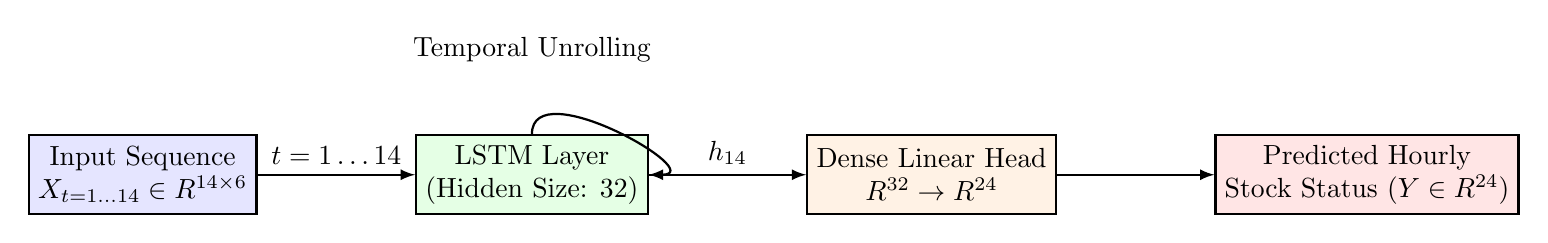
\begin{tikzpicture}[
        node distance=1.5cm and 2cm,
        box/.style={rectangle, draw, thick, minimum width=2.5cm, minimum height=1cm, align=center},
        arrow/.style={-latex, thick}
    ]
    % Nodes
    \node[box, fill=blue!10] (input) {Input Sequence \\ $X_{t=1 \dots 14} \in \mathbb{R}^{14 \times 6}$};
    \node[box, fill=green!10, right=of input] (lstm) {LSTM Layer \\ (Hidden Size: 32)};
    \node[box, fill=orange!10, right=of lstm] (dense) {Dense Linear Head \\ $\mathbb{R}^{32} \rightarrow \mathbb{R}^{24}$};
    \node[box, fill=red!10, right=of dense] (output) {Predicted Hourly \\ Stock Status ($Y \in \mathbb{R}^{24}$)};
    
    % Edges
    \draw[arrow] (input) -- node[above] {$t=1 \dots 14$} (lstm);
    \draw[arrow] (lstm) -- node[above] {$h_{14}$} (dense);
    \draw[arrow] (dense) -- (output);
    
    % Internal LSTM loop indication
    \draw[-latex, thick] (lstm.north) .. controls +(up:0.8cm) and +(right:0.8cm) .. (lstm.east);
    \node[above=0.8cm of lstm] {Temporal Unrolling};
    \end{tikzpicture}
    }
    \caption{The Canonical LSTM processing pipeline for 24-hour stockout prediction.}
    \label{fig:canonical_lstm}
\end{figure}

This Canonical LSTM was much faster (only 19,992 parameters) and slightly more accurate (0.7880 F1-Score). However, it still had a flaw: it forced the LSTM gates to track crazy demand spikes and actual physical inventory limits inside the exact same hidden state $h_t$, which confused the model.

\subsection{Baseline Transformers}
Because everyone uses Transformers nowadays, our team also tested some heavy Transformer models, specifically PatchTST \cite{nie2023patchtst} and Temporal Fusion Transformers (TFT) \cite{lim2021tft}. Even though they were massive (over 280,000 parameters), they actually did worse than our basic LSTM, getting F1-Scores around 0.7540 to 0.7685. Transformers are built to look at everything at once, which didn't fit well with our short 14-day history where physical stock goes down step-by-step. They were just too big for the job.

\begin{figure}[!htbp]
    \centering
    
\includegraphics[width=0.75\textwidth]{../btp-repo/docs/images/hourly_f1_vs_params_by_family.png}
    \caption{Broad comparison across model families, illustrating the parameter-efficiency dominance of recurrent and linear models over Transformers on the FreshRetailNet-50K task.}
    \label{fig:family_comparison}
\end{figure}

\section{Figuring Out Feature Importance}

Early on, our team wondered if we really needed all 13 features the dataset provided. Sometimes giving a model too much messy data just confuses it (which is probably why the Transformers failed). To fix this scientifically, we used a technique called Integrated Gradients (IG) \cite{sundararajan2017ig} to show us exactly what the model was paying attention to over the 14 days.

\begin{figure}[!htbp]
    \centering
    
\includegraphics[width=0.75\textwidth]{../btp-repo/docs/images/ig_heatmap.png}
    
    \vspace{0.5cm}
    \hspace*{-1.2cm}
\includegraphics[width=0.75\textwidth]{../btp-repo/docs/images/ig_barplot.png}
    \caption{Integrated Gradients Heatmap and Feature Importance Barplot revealing the disproportionate importance of recent inventory signals compared to historical static features.}
    \label{fig:ig_heatmap}
\end{figure}

As shown in Figure \ref{fig:ig_heatmap}, this test showed us two really important things that changed how we built the rest of our models:
\begin{enumerate}
    \item \textbf{Recent Data is King:} The data from the last two days ($t=13$ and $t=14$) was way more important than what happened two weeks ago.
    \item \textbf{Inventory Beats Demand:} Hard numbers about how much stock is left (like \texttt{stock\_hour6\_22\_cnt}) were far more useful than messy data about past sales or discounts.
\end{enumerate}

Based on this, our team threw out the bad data and kept only 6 essential features, giving our models a much cleaner signal to learn from.

\section{Building Our Custom LSTMs}

Armed with just the best features, our team started building a custom model piece-by-piece. We tested different structural setups to see what actually improved predictions. Table \ref{tab:rnn_variations} shows the steps we took.

\begin{table}[!htbp]
\centering
\caption{Systematic Progression of Recurrent Architectural Variations}
\label{tab:rnn_variations}
\begin{tabular}{llrr}
\toprule
\textbf{Stage} & \textbf{Architecture} & \textbf{Parameters} & \textbf{F1-Score} \\
\midrule
1 & Baseline SimpleRNN (h=64) & 14,744 & 0.7750 \\
2 & Dual-Stream SimpleRNN & 5,016 & 0.7782 \\
3 & Baseline Vanilla LSTM (h=96) & 44,952 & 0.7852 \\
4 & Feature-Reduced Canonical LSTM (h=32) & 19,992 & 0.7880 \\
5 & \textbf{Dual-Stream Inventory Shortcut LSTM} & \textbf{4,600} & \textbf{0.7941} \\
\bottomrule
\end{tabular}
\end{table}

\subsection{Our Final Custom LSTM: Dual-Stream Inventory Shortcut}

To fix the confusion happening inside the Canonical LSTM, we built our final custom model: the \textbf{Dual-Stream Inventory Shortcut LSTM}. 

We split the 6 good features into two groups: 4 features for Demand, and 2 features for Inventory. We gave each group its own separate LSTM to process. On top of that, because our heatmap showed that the very last day's inventory is the most important thing, we added a special "Shortcut." This shortcut takes the inventory numbers from Day 14 and sends them straight to the final output, completely bypassing the LSTMs. This guarantees that the LSTM never accidentally "forgets" the most important data.

\begin{figure}[!htbp]
    \centering
    \includegraphics[width=0.95\textwidth]{../btp-repo/docs/architecture.jpeg}
    \caption{The Dual-Stream Inventory Shortcut LSTM Architecture. Notice the explicit inventory shortcut preserving the $t=14$ state.}
    \label{fig:dual_stream_lstm}
\end{figure}

This new design dropped the parameter count all the way down to just 4,600, but pushed our F1-Score up to 0.7941, making it our best recurrent model by far.

\begin{figure}[!htbp]
    \centering
    \includegraphics[width=0.85\textwidth]{../btp-repo/docs/images/dualstream_vs_normal_lstm_comparison.png}
    \caption{Architectural Impact: Dual-Stream LSTM vs Normal LSTM Comparison.}
    \label{fig:dualstream_comparison}
\end{figure}

\clearpage
\section{DLinear (Decomposition Linear) Architectures}

After doing everything we could with LSTMs, our team wanted to see if newer Decomposition Linear (DLinear) models could do better. According to Zeng et al. (2023) \cite{zeng2023dlinear}, these simple, single-layer models that split time-series data into Trends and Seasons can sometimes beat complex deep learning models because they are simpler and don't get stuck trying to remember long sequences.

\subsection{Standard DLinear}

Standard DLinear takes the input data $X$ and splits it into a Trend piece ($X_{trend}$, found by averaging recent data) and a Seasonal piece ($X_{seasonal}$, found by subtracting the Trend from the original). The math looks like this:

\begin{align}
    X_{trend} &= \text{AvgPool1D}(X) \\
    X_{seasonal} &= X - X_{trend}
\end{align}

Then, it just uses standard linear layers ($W_{trend}, W_{seasonal}$) to map these pieces directly to the 24-hour prediction. It is very fast and easy to understand:

\begin{equation}
    Y_{pred} = (W_{trend} \cdot X_{trend}) + (W_{seasonal} \cdot X_{seasonal})
\end{equation}

\subsection{Hourly Slot-Specific DLinear}

While Standard DLinear applies a single linear layer to forecast all 24 hours, the \textbf{Hourly Slot-Specific DLinear} maintains 24 dedicated independent projection heads. Because predicting stockouts at 11 AM (lunch rush) involves very different signals than predicting stockouts at 3 PM, using independent weight matrices $W^{h}_{trend}$ and $W^{h}_{seasonal}$ for each hour $h \in \{1, \dots, 24\}$ resolves inter-hour gradient conflicts.

\subsection{Multi-Kernel DLinear}

To make DLinear work even better for the crazy ups and downs of grocery shopping, our team built the \textbf{Multi-Kernel DLinear}. Instead of just doing one average to find the trend, this model runs multiple averages at the same time (like $k=3, 5, 7$) to catch both sudden panic-buying and smooth weekly habits. It groups all these trends together like this:

\begin{equation}
    X_{trend} = \text{Concat}(\text{AvgPool1D}_{k=3}(X), \text{AvgPool1D}_{k=5}(X), \text{AvgPool1D}_{k=7}(X))
\end{equation}

\begin{figure}[!htbp]
    \centering
    \includegraphics[width=0.85\textwidth]{../btp-repo/docs/images/lstm_vs_dlinear_comparison.png}
    \caption{Empirical Benchmark comparing the impact of these architectural advancements.}
    \label{fig:lstm_vs_dlinear_comparison}
\end{figure}

\subsection{Non-Linear DLinear (GELU)}

Standard DLinear is purely linear, which limits its ability to model complex threshold behaviors (e.g., stockouts only trigger when inventory drops below a strict dynamic limit). To solve this, we introduced the \textbf{Non-Linear DLinear with GELU Activation Bottleneck}. 

This variant routes the seasonal and trend components through a multi-layer perceptron (MLP) containing a Gaussian Error Linear Unit (GELU) before producing logits.
\begin{align}
    Y_{seasonal} &= W_{s2}(\text{GELU}(W_{s1} \cdot X_{seasonal})) \\
    Y_{trend} &= W_{t2}(\text{GELU}(W_{t1} \cdot X_{trend})) \\
    Y_{pred} &= Y_{seasonal} + Y_{trend}
\end{align}

Combining all these advancements yields our best model: the Multi-Kernel Non-Linear DLinear.

\begin{figure}[!htbp]
    \centering
    \resizebox{0.9\textwidth}{!}{
    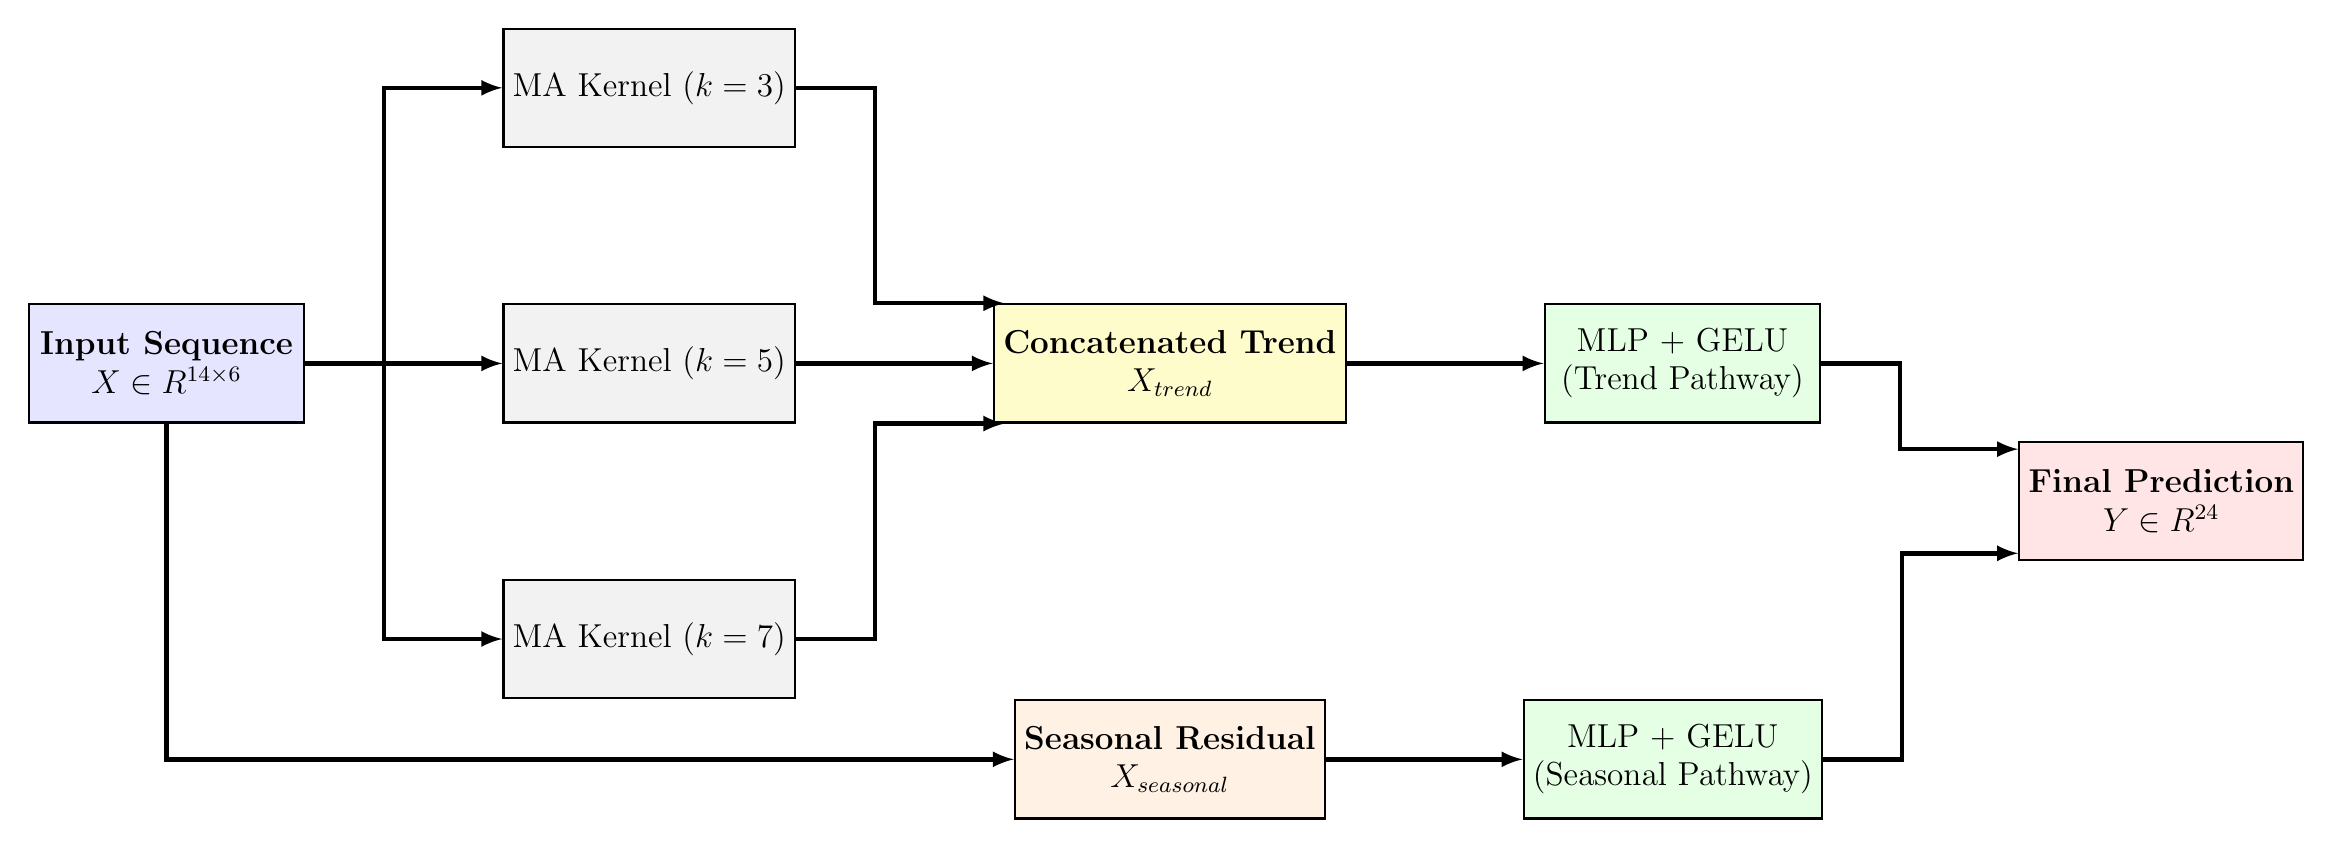
\begin{tikzpicture}[
        node distance=1.5cm and 2.5cm,
        box/.style={rectangle, draw, thick, minimum width=3.5cm, minimum height=1.5cm, align=center, fill=gray!10, font=\large},
        arrow/.style={-latex, ultra thick}
    ]
    % Input
    \node[box, fill=blue!10] (input) {\textbf{Input Sequence} \\ $X \in \mathbb{R}^{14 \times 6}$};
    
    % Decomposition
    \node[box, right=2.5cm of input, yshift=3.5cm] (ma3) {MA Kernel ($k=3$)};
    \node[box, right=2.5cm of input] (ma5) {MA Kernel ($k=5$)};
    \node[box, right=2.5cm of input, yshift=-3.5cm] (ma7) {MA Kernel ($k=7$)};
    
    % Trend Concat
    \node[box, fill=yellow!20, right=2.5cm of ma5] (concat) {\textbf{Concatenated Trend} \\ $X_{trend}$};
    
    % Seasonal
    \node[box, fill=orange!10, below=3.5cm of concat] (seasonal) {\textbf{Seasonal Residual} \\ $X_{seasonal}$};
    
    % GELU Bottlenecks
    \node[box, fill=green!10, right=2.5cm of concat] (gelu_t) {MLP + GELU \\ (Trend Pathway)};
    \node[box, fill=green!10, right=2.5cm of seasonal] (gelu_s) {MLP + GELU \\ (Seasonal Pathway)};
    
    % Output
    \node[box, fill=red!10, right=2.5cm of gelu_t, yshift=-1.75cm] (output) {\textbf{Final Prediction} \\ $Y \in \mathbb{R}^{24}$};
    
    % Edges
    \draw[arrow] (input.east) -- ++(1,0) |- (ma3.west);
    \draw[arrow] (input) -- (ma5);
    \draw[arrow] (input.east) -- ++(1,0) |- (ma7.west);
    
    \draw[arrow] (ma3.east) -- ++(1,0) |- (concat.160);
    \draw[arrow] (ma5) -- (concat);
    \draw[arrow] (ma7.east) -- ++(1,0) |- (concat.200);
    
    % Seasonal is X - ma5 (simplification for diagram)
    \draw[arrow] (input.south) |- (seasonal.west);
    
    \draw[arrow] (concat) -- (gelu_t);
    \draw[arrow] (seasonal) -- (gelu_s);
    
    \draw[arrow] (gelu_t.east) -- ++(1,0) |- (output.160);
    \draw[arrow] (gelu_s.east) -- ++(1,0) |- (output.200);
    \end{tikzpicture}
    }
    \caption{Architecture of the Multi-Kernel Non-Linear DLinear with GELU bottlenecks.}
    \label{fig:multi_kernel_nonlinear_dlinear}
\end{figure}
\label{chap:methodology}
\clearpage
\thispagestyle{empty}
\newpage

\chapter{Tasks Completed}
\label{chap:tasks}

To find the best model for this project, our team followed a strict three-month plan. Here is a breakdown of what we accomplished each month:

\begin{enumerate}
    \item \textbf{Month 1: Research and Setting Up the Basics} 
    
    \begin{itemize}
        \item We started by researching older forecasting methods to understand how inventory prediction used to be done.
        \item We cleaned up the FreshRetailNet-50K dataset and organized it so our models could read it.
        \item We built and trained basic Vanilla RNN and Vanilla LSTM models to see how they performed, which gave us a baseline to beat (44K parameters, 0.785 F1-Score).
    \end{itemize}
    
    \item \textbf{Month 2: Feature Engineering and Building Our Custom Model}
    
    \begin{itemize}
        \item We used Integrated Gradients to figure out which features actually mattered, and threw away the bad ones, leaving us with just 6 strong features.
        \item We designed a new "Dual-Stream" setup that processes crazy demand spikes separately from hard inventory facts.
        \item We finished building our custom \textit{Dual-Stream Inventory Shortcut LSTM}, which shrank the model down to just 4,600 parameters while actually beating the bigger baseline models.
    \end{itemize}
    
    \item \textbf{Month 3: Testing Linear Models and Final Results}
    
    \begin{itemize}
        \item We set up a very strict testing process (using Focal Loss and dynamic threshold scanning) to make sure our results were completely fair and accurate.
        \item We built and tested the \textit{Multi-Kernel DLinear} model to see if it could handle both sudden panic-buying and longer weekly trends.
        \item We collected all our final numbers, created the graphs, proved that the Multi-Kernel DLinear was our best model, and wrote this final thesis report.
    \end{itemize}
\end{enumerate}
\label{chap:tasks}
\clearpage
\thispagestyle{empty}
\newpage

\chapter{Results and Conclusion}
\label{chap:results}

As our project went on, we knew we had to compare our custom LSTM models against the newest linear models to see which was truly better. This chapter explains how we tested everything fairly, shows our final numbers, and gives our overall conclusion.

\section{Standardized Evaluation Framework}

To make sure we were comparing apples to apples, our team set up a very strict testing process. This stopped any model from looking better just because of lucky guesses or messy data:

\begin{itemize}
    \item \textbf{Dataset Scope:} We only tested the top 15 busiest store-product combinations. This stopped the models from learning useless patterns from items that never sell anyway.
    \item \textbf{Holdout Strategy:} We used a strict timeline split. We hid the last 15 days of the dataset from the models completely, and only used those days for the final test.
    \item \textbf{Optimization:} In retail, stockouts don't happen as often as regular sales. To fix this imbalance, we trained the models using \textbf{Focal Loss} instead of standard Binary Cross-Entropy. The Focal Loss is defined mathematically as:
    \begin{equation}
        FL(p_t) = -\alpha_t (1 - p_t)^\gamma \log(p_t)
    \end{equation}
    where $p_t$ is the model's estimated probability for the stockout class. We configured the focusing parameter $\gamma = 2.0$ and the balancing factor $\alpha = 0.5$.
    \item \textbf{Dynamic Thresholding:} Instead of just picking a standard 50/50 cutoff for predictions, we had the computer scan all cutoffs from 10\% to 90\% on a practice set to find the perfect spot that maximized the F1-Score.
\end{itemize}

\section{Final Empirical Results}

We tested our main recurrent models against a few versions of the DLinear architecture (which we talked about in Chapter 4). You can see the final scores and how big each model is in Table \ref{tab:final_variants}.

\begin{table}[!htbp]
  \centering
  \small
  \caption{Master Empirical Validation Leaderboard}
  \label{tab:final_variants}
  \resizebox{\textwidth}{!}{
  \begin{tabular}{llccccc}
    \toprule
    \textbf{Rank} & \textbf{Architecture Name} & \textbf{Category} & \textbf{Params} & \textbf{F1-Score} & \textbf{Recall} & \textbf{MAE (hrs)} \\
    \midrule
    \textbf{1} & \textbf{Multi-Kernel Non-Linear DLinear} & Non-Linear DLinear & 42,339 & \textbf{0.8156} & 87.13\% & \textbf{3.75} \\
    \textbf{2} & \textbf{Multi-Kernel Linear DLinear} & Linear (Multi-Scale) & 13,539 & \textbf{0.8131} & 85.22\% & 3.86 \\
    \textbf{3} & \textbf{Non-Linear GELU DLinear} & Non-Linear DLinear & 21,168 & \textbf{0.8083} & \textbf{91.37\%} & 4.20 \\
    4 & Hourly Slot-Specific DLinear & Linear (24 Heads) & 6,744 & \textbf{0.8058} & 88.02\% & 4.23 \\
    5 & Standard Linear DLinear & Linear (Decomp) & 6,768 & \textbf{0.7932} & 87.44\% & 4.28 \\
    6 & Dual-Stream Inventory Shortcut & LSTM Family & 4,600 & \textbf{0.7926} & 80.79\% & 3.96 \\
    \textbf{Base} & \textbf{Best Normal LSTM (h=32)} & Normal LSTM & 5,912 & \textbf{0.7897} & 81.29\% & 4.31 \\
    7 & Feature-Reduced Standard LSTM & Normal LSTM & 19,992 & 0.7880 & 81.60\% & 4.58 \\
    8 & Baseline Standard LSTM (h=96) & Normal LSTM & 44,952 & 0.7852 & 80.40\% & 4.67 \\
    9 & Vanilla Simple RNN (h=64) & RNN Family & 14,744 & 0.7750 & 81.02\% & 4.23 \\
    10 & PatchTST Patch Linear & Transformer & 285,624 & 0.7540 & 81.90\% & 4.16 \\
    \bottomrule
  \end{tabular}
  }
\end{table}

\begin{figure}[!htbp]
    \centering
    \includegraphics[width=0.75\textwidth]{../btp-repo/docs/images/nonlinear_dlinear_comparison.png}
    \caption{Final Empirical Comparison: The linear architectures systematically outperform the recurrent LSTM bounds.}
    \label{fig:final_comparison}
\end{figure}

The numbers clearly showed that the \textbf{Multi-Kernel Non-Linear DLinear} was the overall winner. It hit a peak F1-Score of \textbf{0.8156} and a remarkably low MAE of \textbf{3.75 hours} while using 42,339 parameters. Additionally, the \textbf{Non-Linear GELU DLinear} achieved a record-setting Stockout Recall of \textbf{91.37\%}, making it ideal for strict risk mitigation scenarios. It comprehensively beat both our custom LSTM and all the basic baseline models (as you can see in Figure \ref{fig:final_comparison}). 



\section{Conclusion}

This project took on the real-world problem of predicting hourly stockouts in fast-paced grocery delivery. By moving away from predicting daily totals and focusing on specific hour-by-hour predictions, our team tackled a problem that actually costs delivery apps a lot of customers.

Going through all these different models taught our team a few big lessons:

\begin{enumerate}
    \item \textbf{Good Features Matter Most:} Getting rid of bad data and focusing on a few strong features helped the models way more than just making the models bigger.
    \item \textbf{Routing the Data Helps:} When building LSTMs, separating the demand numbers from the inventory numbers, and taking a "shortcut" for the most recent day's data, stopped the model from forgetting the important stuff.
    \item \textbf{Linear Models Win Here:} In our strict testing, we proved that simple Decomposition Linear (DLinear) models are actually better for this specific short-term forecasting job than complex deep learning LSTMs.
\end{enumerate}

While our Dual-Stream Inventory Shortcut LSTM was our best idea for a recurrent model, the \textbf{Multi-Kernel Non-Linear DLinear} is the final model we recommend using in the real world. Because it doesn't have messy recurrent memory, it leverages independent GELU bottlenecks and runs multiple averages at the same time to easily handle the short 14-day history. This allows it to catch both sudden panic-buying and smooth weekly trends to get the highest F1-Score of 0.8156 and lowest MAE of 3.75 hours. 

By predicting exactly which hour a shelf will empty, this tool can help grocery managers restock shelves before they run out. This means less spoiled food, less wasted money, and happier customers when they open the app to order.
\label{chap:results}
\clearpage
\thispagestyle{empty}
\newpage 

\addtocounter{page}{-1}

%************************************************ BEGIN REFERENCES **********************************************
\renewcommand{\bibname}{References}
\bibliographystyle{ieeetr}
\nocite{*}
\bibliography{references}
\addcontentsline{toc}{chapter}{References} % Removed as per supervisor feedback

%%%..........................................................................................................................................
%\fancychapter{Appendix}\label{Sunil_Appendix}
%\chapter{Appendix}\label{Sunil_Appendix}
%  \include{Chapters/Appendix/Appendix}
%\clearpage
%%..........................................................................................................................................
%\fancychapter{Cepstral Analysis}
%\label{app:lpc}
%\include{chapters/Appendix/CFA}
%\clearpage
%%..........................................................................................................................................
%\fancychapter{Linear Prediction Coefficients Computation}
%\label{app:sine}
%\include{chapters/Appendix/Appendix_lpc_V2}
%\clearpage
%%..........................................................................................................................................
%\fancychapter{Composite Objective Quality Measures}
%\label{app:cqm}
%\include{Chapters/Appendix/Appendix_cqm_V1}
%\clearpage
%%..........................................................................................................................................
%\fancychapter{MFCC Feature Extraction}
%\label{app:mfcc}
%\include{Chapters/Appendix/Appendix_mfcc_V1}
%\clearpage
%%..........................................................................................................................................
%\fancychapter{Gaussian Mixture Models}
%\label{app:gmm}
%\include{Chapters/Appendix/Appendix_gmm_V1}
%\clearpage
%..........................................................................................................................................
%\doublespacing
%\normalsize
%\pdfbookmark{Publications}{Publications}
%\fancyhead[LE]{\bfseries\small{List of Publications}}
%\fancyhead[RO]{\bfseries\small{List of Publications}}
%\pdfbookmark[1]{List of Publications}{los}
%\addstarredchapter{List of Publications}
%\include{FrontPages/publ}
%\clearpage

%% LIST OF SYMBOLS
%\fancyhead[LE]{\bfseries\small{List of Symbols}}
%\fancyhead[RO]{\bfseries\small{List of Symbols}}
%\pdfbookmark[1]{List of Symbols}{los}
%\addstarredchapter{List of Symbols}
%\include{FrontPages/Symbols}
%\clearpage
%******************************************************************************************************************************************************************

\end{document}
